\documentclass[11pt,compress,t,notes=noshow, aspectratio=169, xcolor=table]{beamer}

\usepackage{../../style/lmu-lecture}
% Defines macros and environments
% This file is included in slides and exercises

% Rarely used fontstyle for R packages, used only in 
% - forests/slides-forests-benchmark.tex
% - exercises/single-exercises/methods_l_1.Rnw
% - slides/cart/attic/slides_extra_trees.Rnw
\newcommand{\pkg}[1]{{\fontseries{b}\selectfont #1}}

% Spacing helpers, used often (mostly in exercises for \dlz)
\newcommand{\lz}{\vspace{0.5cm}} % vertical space (used often in slides)
\newcommand{\dlz}{\vspace{1cm}}  % double vertical space (used often in exercises, never in slides)
\newcommand{\oneliner}[1] % Oneliner for important statements, used e.g. in iml, algods
{\begin{block}{}\begin{center}\begin{Large}#1\end{Large}\end{center}\end{block}}

% Don't know if this is used or needed, remove?
% textcolor that works in mathmode
% https://tex.stackexchange.com/a/261480
% Used e.g. in forests/slides-forests-bagging.tex
% [...] \textcolor{blue}{\tfrac{1}{M}\sum^M_{m} [...]
% \makeatletter
% \renewcommand*{\@textcolor}[3]{%
%   \protect\leavevmode
%   \begingroup
%     \color#1{#2}#3%
%   \endgroup
% }
% \makeatother

\newcommand{\open}{}
\newcommand{\close}{}

\title{Interpretable Machine Learning}
% \author{LMU}
%\institute{\href{https://compstat-lmu.github.io/lecture_iml/}{compstat-lmu.github.io/lecture\_iml}}
\date{}

\begin{document}

%Gliederung:
%- Intro with examples, motivation, problems
%- fANOVA calculation + example
%- conditions + theory
%- other methods (gen fANOVA, ALE)

\newcommand{\titlefigure}{figure/open_blackbox}
\newcommand{\learninggoals}{
\item Basic idea of additive functional decompositions
\item Motivation and usefulness of functional decompositions
\item Difficulty of obtaining or even defining a functional decomposition}

\lecturechapter{Introduction to Functional Decomposition}
\lecture{Interpretable Machine Learning}


\begin{frame}{Recap: interaction}
    Recap: Interactions between features: The effect of some features on the prediction output depends on (one or more) other features \\
    This cannot be captured by the main feature effects alone (i.e. by a GAM).
    We want to know, which parts are attributed to effects of single features (s.o. feature effect methods), and which to interactions.

    \textit{TO DO: After introducing PDPs and PD-functions more generally in chapter 3, we would want to introduce H-statistic as a measure / as a possible definition for interactions, maybe even in the general case (i.e. the H-statistic for testing for an \(n\)-way interaction between \(n\) many features).}

\end{frame}

\begin{frame}{First Example: Additive decomposition}

    \begin{example}

        The function \( \fh(x_1, x_2) = 4 - 2x_1 + 0.3 e^{x_2} + |x_1|x_2 \) depends on two features, and contains the interaction \( |x_1|x_2 \) between the two features.
    
        [visualization] 

        Using a GAM or looking at the effects of single features will not allow us to fully understand the function. But from the formula, we can additively decompose this function, depending on the degree of interaction:

        \begin{equation}\label{eq1}
            \begin{split}
                g_0(x_1, x_2) = 4 &  \text{ Everything depending on no features at all}  \\
                \begin{split}
                    g_1(x_1, x_2) = 2x_1 \\
                    g_1(x_1, x_2) =  0.3 e^{x_2}
                \end{split}
                    & \text{ Parts depending on a single feature (main effects)}  \\
                g_{1,2}(x_1, x_2) = |x_1|x_2 & \text{ Part depending on both features (interaction)}  \\
            \end{split}
        \end{equation}
        
        The single terms enable immediate interpretation (effects of single features, single interactions etc). \\
    
    \end{example}

    
    
\end{frame}

\begin{frame}{First Example: Additive decomposition}

    In general, functional form is unknown, but goal is to find such a decomposition:
    Given a function (or a model) \(\fh: \R^2 \to \R\), we want to find a decomposition

    \begin{equation}
        \fh(x_1, x_2) =  g_{0} + g_1(x_1) + g_2(x_2) + g_{\open 1, 2 \close}(x_1, x_2)
    \end{equation}
    
\end{frame}

\begin{frame}{Another example}

    \begin{example}

        Consider the function

        \begin{equation*}
            \fh(x_1, x_2, x_3) = - 2x_1 - 2\sin(x_3) + |x_1|x_2 + 0.5 x_1 x_2 x_3 - \sin(x_2 x_3) +1
        \end{equation*}

        We can again find the additive decomposition by reading from the functional formula, but some terms are empty, because certain types of effects and interactions are not present:

        [...]

        \(\Rightarrow\) 8 components in total
        
    \end{example}
    
\end{frame}

\begin{frame}{General Form of Functional Decomposition
%\\
%\citebutton{Sobol (1993)}{http://www.andreasaltelli.eu/file/repository/sobol1993.pdf}
% \citebutton{Sobol (2003)}{https://doi.org/10.1016/S0951-8320(02)00229-6}
%\citebutton{Li et al. (2001)}{https://doi.org/10.1021/jp010450t}
\citebutton{Li and Rabitz (2011)}{https://doi.org/10.1007/s10910-011-9898-0}
\citebutton{Chastaing et al. (2012)}{https://doi.org/10.1214/12-EJS749}
}

%\textbf{High-Dimensional Model Representation (HDMR):} 
For interpretation purposes, one might be interested in decomposing a square-integrable function $\fh: \R^p \mapsto \R$ into sum of components of different dimensions w.r.t. inputs $x_1, \ldots, x_p$: %
\begin{equation*}
\begin{split}
\fh(\xv) =  %g_{\open \emptyset \close} +
\textstyle\sum_{S \subseteq \{1,\ldots,p\}} g_{S}(\xv_S) = \; & g_{\open \emptyset \close} + g_{\open 1 \close}(x_1) + g_{\open 2 \close}(x_2) + \dots + g_{\open p \close}(x_p) + \\
& g_{\open 1, 2 \close}(x_1, x_2) + \dots + g_{\open p-1, p \close}(x_{p-1}, x_p) + \dots + \\
& g_{\open 1,\ldots,p \close}(x_1, \ldots, x_p)
\end{split}
\end{equation*}
%\vspace{-5pt}%\pause
where 
\begin{itemize}
\item $g_{\open \emptyset \close} \hat = $ Constant mean (intercept) %$\mathbb{E}_X (\fh(\xv)) $
\item $g_{\open j \close} \hat = $ first-order or main effect of $j$-th feature alone on $\fh(\xv)$
%\item Bivariate terms $g_{\open j, k \close} \hat = $ second-order effect of features $j$ and $k$ w.r.t. $\fh(\xv)$%, etc.
\item $g_{S}(\xv_S) \hat = $ $|S|$-order effect, depends \textbf{only} on features in $S$ %$x_j$ for all $j \in S$
\end{itemize}
\lz

%High-Dimensional Model Representation (HDMR)
%Functional ANOVA decomposition
%Sobol-Hoeffding decomposition
\end{frame}

\begin{frame}{Recap: GAM}

    Compare to GAM: The same decomposition is used, but in case of GAM, no interactions at all are considered, only main effects. I.p. any GAM already comes with its decomposition! \\
    Same for linear models / linear regression and GLMs.
    
\end{frame}

\begin{frame}{Functional Decomposition -- Example}
\textbf{Example:} $\fh(\xv) = 2 + x_1^2 - x_2^2 + x_1 \cdot x_2$ (e.g., if $x_1 = 5$ and $x_2 = 10$ $\Rightarrow$ $\fh(\xv) = -23$)

\begin{itemize}
    \item Computation of components using feature values $x_1 = x_2 = (-10, -9, \ldots, 10)^\top$ gives:
    \begin{columns}[c, totalwidth=\linewidth]
    \begin{column}{0.75\textwidth}
        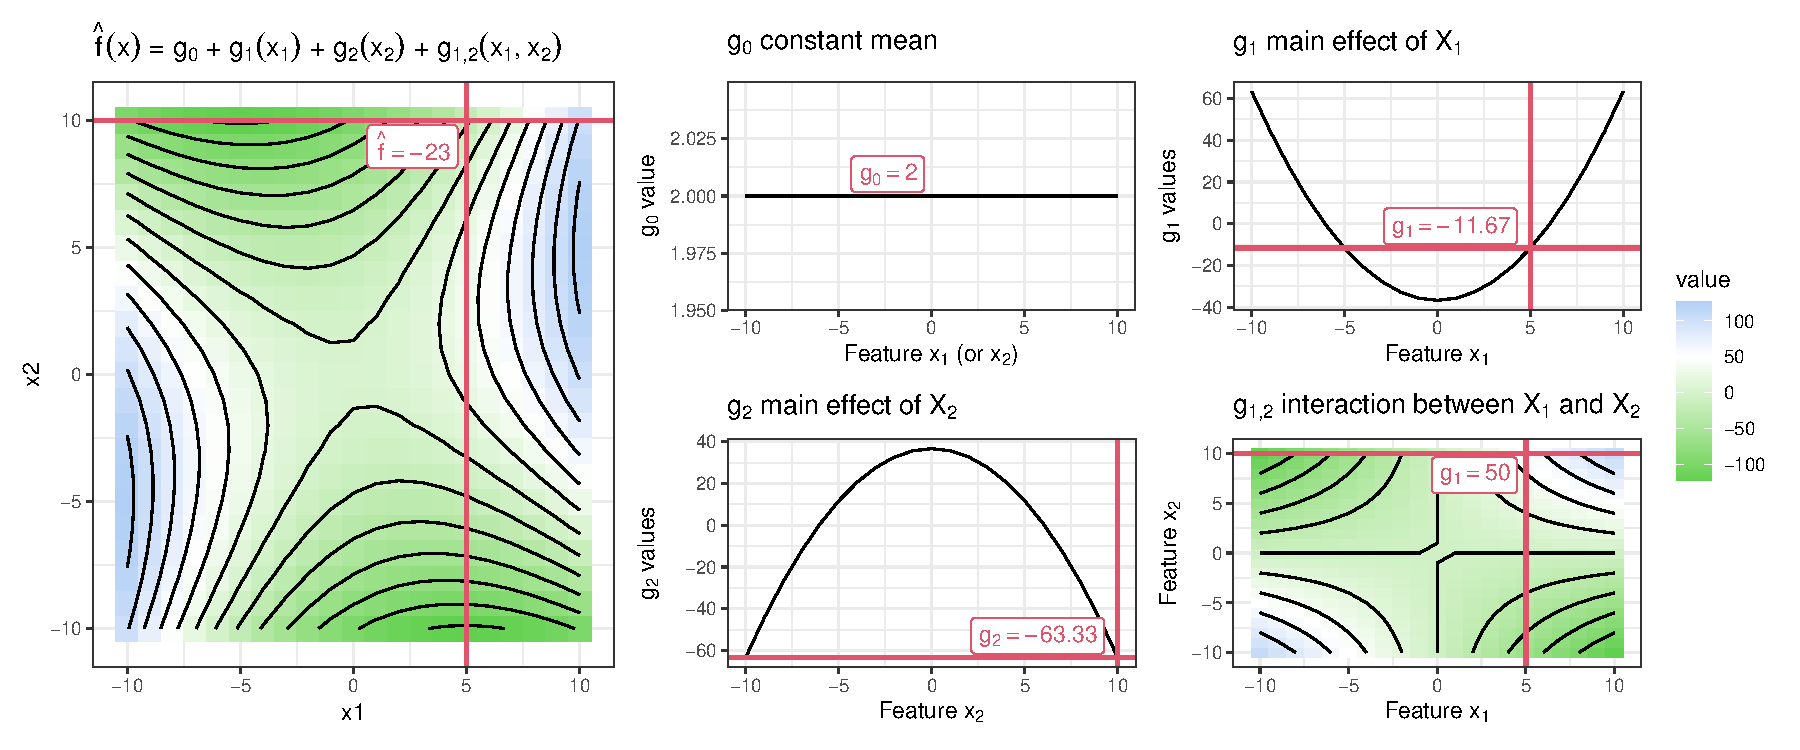
\includegraphics[width = \textwidth]{figure/decomposition}
    \end{column}
    \begin{column}{0.25\textwidth}
    For $x_1 = 5$ and $x_2 = 10$:\\
    \begin{itemize}
        \item $g_{\open \emptyset \close} = 2$
        \item $g_{\open 1 \close}(x_1) = -9.67$
        \item $g_{\open 2 \close}(x_2) = -65.33$
        \item $g_{\open 1,2 \close}(x_1, x_2) = 50$
        \item[$\Rightarrow$] $\fh(\xv) = -23$
    \end{itemize}
    \end{column}
    \end{columns}
\pause
    \item Vanishing condition means:
    \begin{itemize}
        \item $g_1$ and $g_2$ are mean-centered w.r.t. marginal distribution of $x_1$ and $x_2$
        \item Integral of $g_{1,2}$ over marginal distribution $x_1$ (or $x_2$) is always 0.
        %, i.e., for each slice at $x_1$ (and $x_2$), the integral of $g_{1,2}$ 
    \end{itemize}
\end{itemize} 
\end{frame}

\begin{frame}{??}
    Super nice and extremely powerful decomposition! "Holy Gral of interpreting complex models"\\
    BUT 2 Problems:
    \begin{itemize}
        \item Definition not complete, such decomposition is not unique, and many trivial decompositions are not useful at all (see next slide) \\
            This problem get's much worse, whenever features are not independent \\
        \textbf{N.B.:} %Further constraints are required to obtain an unique and optimal solution for the components
        A unique solution for the components only exists under certain assumptions
        %and constraints
        %independent inputs and a \textit{vanishing condition}
        %$$\mathbb{E}_{X_j} (g_{S}(\xv_S)) = \int g_{S}(\xv_S) d \mathbb{P}(x_j) = 0, \forall j \in S, \forall S \subseteq \{1, \ldots, p\}$$
        %Without further constraints on components, there is no unique solution.
        %\end{itemize}
        \item Calculating such a decomposition is super, super hard in practice \\
            See for example: For \(p\) features, the decomposition has \(2^p\) terms \(\Rightarrow\) not very meaningful to interpret so many different terms \\
    \end{itemize}
\end{frame}

\begin{frame}{Problem of Definition}

    [an example showing that constraints are needed]
    \\
    \(\Rightarrow\) The formula from above do not define a unique decomposition, and we need more requirements / constraints to uniquely define a decomposition that is meaningful
    \\
    This problem get's even worse once features are dependent or correlated \(\Rightarrow\) see later
    
\end{frame}

\begin{frame}{Example: Decision Trees}

    [show that one decision tree directly comes with its functional decomposition using indicator functions]\\

    Problem again is uniqueness? If only reading from decision tree using indicator functions, lower-order effects may be hidden inside higher-order terms? \\

    [Example for that, could also be used to explain necessity of constraints / problem of non-uniqueness]\\

    \(\Rightarrow\) Solution for that in 
    \citebutton{Yang (2024)}{https://arxiv.org/abs/2410.19098} \(\Rightarrow\) Too complicated? Rather explain this in constraint-chapter or in other methods-chapter?
    
\end{frame}

\begin{frame}{High-dimensional modl representation (HDMR)}
    [explain link to HDMR?? Or at end of chapter ?]
\end{frame}








\endlecture
\end{document}
